\documentclass{article}
%\documentclass{standalone}

\usepackage[compat=1.1.0]{tikz-feynman}
\usepackage{polski}

\usepackage{pgfplots}
\pgfplotsset{compat=1.18}
\usepackage{amsfonts}
\usepackage{amsmath}

\begin{document}

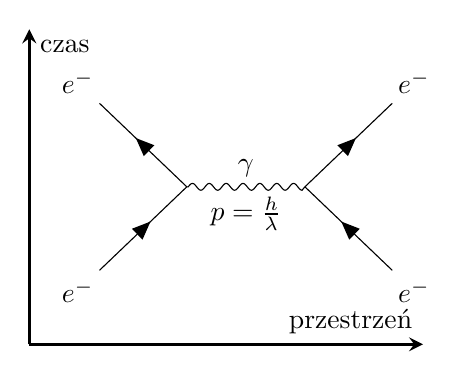
\begin{tikzpicture}
	\draw[very thick,-stealth] (-2,-2) to (-2,2)node[anchor=north west] {czas};
	\draw[very thick,-stealth] (-2,-2) to (3,-2)node[anchor=south east] {przestrzeń};

	\begin{feynman}
		\vertex(a);
		\vertex[above left=of a] (b) {$e^-$};
		\vertex[below left=of a] (d) {$e^-$};
		\vertex[right=of a] (e);
		\vertex[above right=of e] (c) {$e^-$};
		\vertex[below right=of e] (f) {$e^-$};

		\diagram *{
		(d) -- [fermion] (a) -- [fermion] (b),
		(f) -- [fermion] (e) -- [fermion] (c),
		(a) -- [photon, edge label=$\gamma$, edge label'={$p=\frac{h}{\lambda}$}] (e)
		};

	\end{feynman}
\end{tikzpicture}

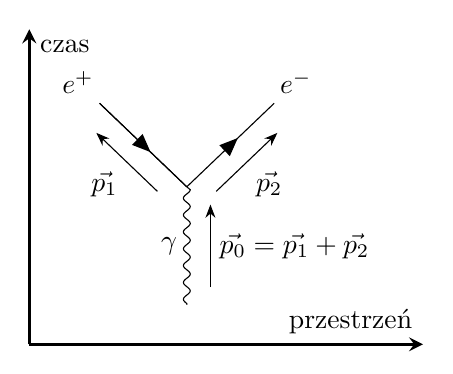
\begin{tikzpicture}
	\draw[very thick,-stealth] (-2,-2) to (-2,2)node[anchor=north west] {czas};
	\draw[very thick,-stealth] (-2,-2) to (3,-2)node[anchor=south east] {przestrzeń};

	\begin{feynman}
		\vertex(a);

		\vertex[below=of a] (b);
		\vertex[above right=of a] (c) {$e^-$};
		\vertex[above left=of a] (d) {$e^+$};

		\diagram *{
		(b) -- [photon, edge label=$\gamma$, momentum'={$\vec{p_0}=\vec{p_1}+\vec{p_2}$}] (a),
		(a) -- [fermion, momentum'={$\vec{p_2}$}] (c),
		(d) -- [fermion] (a),
		(a) -- [momentum={$\vec{p_1}$}](d)
		};

	\end{feynman}
\end{tikzpicture}

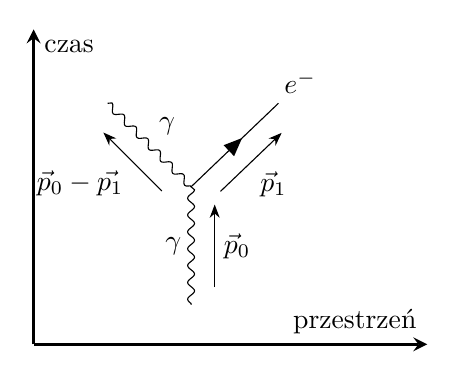
\begin{tikzpicture}
	\draw[very thick,-stealth] (-2,-2) to (-2,2)node[anchor=north west] {czas};
	\draw[very thick,-stealth] (-2,-2) to (3,-2)node[anchor=south east] {przestrzeń};

	\begin{feynman}
		\vertex(a);

		\vertex[below=of a] (b);
		\vertex[above right=of a] (c) {$e^-$};
		\vertex[above left=of a] (d);

		\diagram *{
		(b) -- [photon, edge label=$\gamma$, momentum'={$\vec{p}_0$}] (a),
		(a) -- [fermion, momentum'={$\vec{p}_1$}] (c),
		(a) -- [photon, edge label'={$\gamma$}, momentum={$\vec{p}_0-\vec{p_1}$}](d)
		};

	\end{feynman}
\end{tikzpicture}
\newline

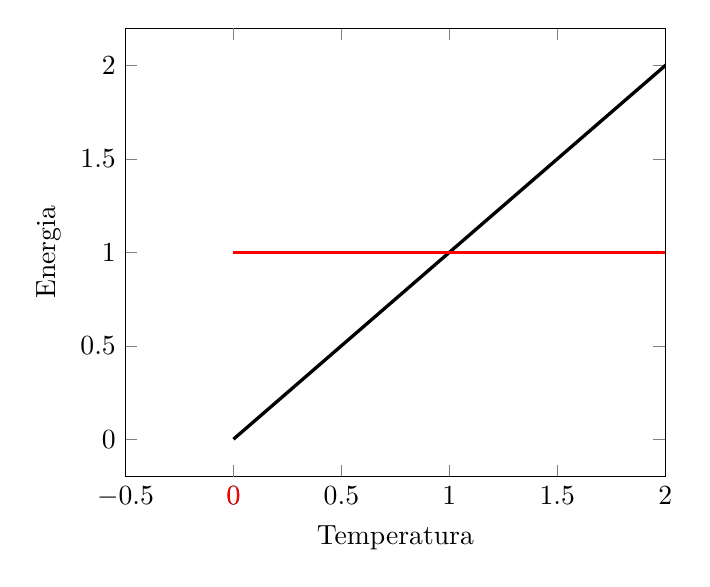
\begin{tikzpicture}
	\begin{axis}[xlabel={Temperatura}, ylabel={Energia}, scale=1, xmin=-0.5,xmax=2, domain=0:4,
			extra x ticks={0}, extra x tick style={red},
			%,xtick={3},xticklabels={$t^*$}
		]

		\addplot[very thick, black, domain=0:4] {
			x >=0 ? x : 0
		};
		\addplot[black,very thick,red]{
			1
		};

	\end{axis}
\end{tikzpicture}

\end{document}